\documentclass[12pt,english]{article}
\usepackage[utf8]{inputenc}
\usepackage{hyperref}
\usepackage[top=1in, bottom=1in, left=1in, right=1in]{geometry}
\usepackage{appendix}

\usepackage[authoryear, round]{natbib}
\usepackage{graphicx}
\usepackage{setspace}
\usepackage{float}

\linespread{2}

\begin{document}
\begin{singlespace}
\title{Predicting Movie Outcomes by Pre-production Characteristics}
\end{singlespace}

\author{Audrey Hopewell\thanks{Department of Economics, University of Oklahoma.\
E-mail~address:~\href{mailto:audrey.hopewell@ou.edu}{audrey.hopewell@ou.edu}}}
\date{May 4, 2020}




\maketitle
\begin{singlespace}
\begin{abstract}
    This paper uses six machine learning algorithms to predict movie success using pre-production characteristics. Movie success is defined as the relationship between revenue and audience reception, which is operationalized as user-generated 1-10 ratings. Movies are classified using two different methods: an ``intuitive" manual classification scheme using the mean of each outcome variable to split the data into quadrants, and k-means clustering. Then, the six machine learning algorithms perform multi-class classification for both types of classification methods. I find that the classes generated by k-means clustering facilitate more accurate predictions than ``intuitive" classes and that the support vector machine is the most successful algorithm for this method.
\end{abstract}
\end{singlespace}

\newpage
\section{Introduction}
The great writer and director Sidney Lumet writes in ``Making Movies" that ``I don't know what makes a hit. I don't think anyone does" \citep[pp. 198]{lumet}. This sentiment might be familiar to anyone who spends \$10 on a ticket to see a movie starring their favorite actor, directed by a lauded filmmaker, for which the trailer looked fascinating, and ends up wanting their money and time back. Conversely, some movies that flop in theaters are revered as masterpieces of the craft. If even experts like Lumet don't know what makes a good movie, perhaps there is a chance for data analysis to shed some light on the relationship between the movie itself and its performance.

This project is inspired by FiveThirtyEight's \href{https://fivethirtyeight.com/tag/hollywood-taxonomy/}{Hollywood Taxonomy series}, in which an actor's movies are classified into three to five categories by plotting their box office gross revenue against their Rotten Tomatoes rating. This results in categories like ``The Most Cowbells" for Will Ferrell (high grossing and highly-rated, such as The LEGO Movie) and ``Hope Sinks" for Sandra Bullock (low grossing and low-rated, such as Miss Congeniality 2) \citep{ferrell, bullock}. 

These categories are humorous and provide retrospective insight, but is there a way to make this concept more useful? For example, is there something about these movies themselves (i.e. their characteristics before they are filmed, edited, and released) that predicts which category they'll fit into? Does a certain genre tend to produce beloved but unprofitable cult classics or box office smashes with terrible reviews, for example? If so, knowing these characteristics could help moviemaking professionals (actors, editors, production designers, etc.) or investors predict a movie's likely performance (in revenue and audience reception) and thus make more informed employment or funding decisions.

\section{Literature Review}
Previous research in the machine learning, management sciences, and economics fields has examined the relationship between movie profitability and movie characteristics. Such research has addressed both movie metadata (such as genre, budget, etc.) and more sophisticated metrics (such as measures of the social networks and expertise of a movie's cast and crew). Key factors in movie success have been defined as audience-based (such as movie reviews or social media sentiment), release-based (such as the number of theaters a movie is released in or the time of year of release), and movie-based (characteristics of the film itself, such as genre and cast information) \citep{lash}. Movie-based characteristics are the only ones available before release, and only a subset of that information is available before a movie is made (e.g. the run time or MPAA rating is not known until the movie has been produced).

In machine learning, the research typically focuses on predicting the success of a movie based on its characteristics. Sharda \& Delen, for example, take a classification approach, using pre-release characteristics and a neural network to predict which of nine revenue-based categories into which a movie will fall \citep{sharda}. Parimi \& Caragea expand this work by including network-based features for revenue classification to account for the dependencies among movie outcomes, e.g. the effect of a star director or actor \citep{parimi}. Lash \& Zhao take a similar approach of using pre-release characteristics--including novel network measures like the ``genre expertise" of a cast weighted by each cast member's "star power" (i.e. average profitability) and actor-director collaboration frequency--but focus on predicting movie profitability and return-on-investment (ROI) rather than revenue, with the goal of constructing a tool for investors to make funding decisions \citep{lash}. Other work, such as that by Elberse, finds that major casting announcements--a pre-production factor--are important drivers of both immediate movie valuation and theater revenue \citep{elberse}. 

Some innovations in the literature include the use of novel measures of star power, movie content, or cultural ``hype" around a film. Apala et al, for example, mine data from social media and use the number of director and cast Twitter followers, the number of trailer views and comments on YouTube, and a sentiment analysis of those YouTube comments to predict movie revenues \citep{apala}. Eliashberg et al use a kernel approach to analyze movie scripts, and using this and estimated production budget (capturing only features known when a movie is ``green-lit"), are able to predict box office revenue more accurately than other measures \citep{eliashberg}. 

Movie success is typically measured by revenue \citep{apala, parimi, simonoff, gopinath, sharda, elberse, eliashberg}. However, some research has used profit or return-on-investment (ROI) as an alternative measure that is meant to be more relevant to investors \citep{lash}. In non-machine learning literature (e.g. management or organizational sciences, who are more focused on the nature of creative processes and success), movie success is measured by individual or collective awards won by the cast and crew \citep{cattani}. Machine learning literature has not typically incorporated this measure directly as a dependent or independent variable, as "star power" measures usually include revenue/profit metrics or social media following \citep{lash, sharda}. 

There is a lack of literature focusing on audience reception as an output. While some \citep{apala} use audience reception as a predictor of movie revenue, the literature typically treats audience opinion as an input to financial indicators rather than something that itself can be predicted or is an outcome of interest. Intuitively, movie professionals are likely interested in audience and peer perception just as much as they are in movie revenue or profit, as movie reception speaks more directly to their talent than revenue or profit, which may simply reflect the size of the advertising budget.

Indeed, Hollywood is a highly reputation-based industry. A history of appearing in well-received and profitable films positively affects an actor's ability to negotiate for future desired projects \citep{ebbers}. Additionally, there is a positive feedback loop, as professional crew members with a history of award success tend to work with other frequently-award professionals and produce more creatively-lauded films \cite{cattani}. Thus, it is in a movie professional's interest to sign on to films that will be creatively well-received, in addition to being profitable.

Even more basically, a strong reputation of creative success is necessary in forming the kinds of social networks that facilitate sustainable employment in the movie industry. Hollywood has been characterized as a project-based industry because each film is made by a novel group of cast and crew. The film itself is a project firm because it comes together, creates an output, and then dissolves \cite{ferriani, jones}. Project firms form largely based on social network connections, which allow information--particularly about skill and reputation--to travel between nodes (individuals in the network) \citep{jones}. Thus, a history of working on movies that are creative successes will facilitate continued employment. Given this industry structure, how should a Hollywood professional navigate which projects to seek employment with, given only the basic information that would be available before a has a full cast and crew and begins production?


\section{Data}
This paper uses a \href{https://www.kaggle.com/rounakbanik/the-movies-dataset#movies_metadata.csv}{dataset} from Kaggle which includes movie metadata compiled from GroupLens and TMDB. The dataset includes metadata for each of 45,000 movies released during or before July 2017. In this case, metadata is basic information about the film, such as its budget, which series it belongs to (e.g. a Bond movie or Toy Story), applicable genres, and more. The dataset also includes quality ratings (and number of ratings) for each movie from 270,000 users for a total of 26 million individual ratings. Ratings range from 1-10. For a complete list of variables, see Appendix A. 

The data require minimal cleaning: certain unneeded variables (such as links to images of movie posters) were removed; character variables were cleaned by removing punctuation, additional words (such as ``name:" preceding each genre) and their numeric identifiers so that only the name of each genre remained. I converted the released date from a factor variable to a Date object and converted budget and revenue to numeric values. I also removed movies that had missing rating or revenue information or had budget values of 0 (which might indicate missing budget information).

Finally, I filtered the dataset to include only a subset of movies that could be considered relevant to the research question and avoid too many confounding variables. I wanted to capture what would be considered ``Hollywood" (or at least Hollywood-adjacent) films that would get a mainstream, theater release. To do so, I omitted movies that are considered "adult", movies not in English (some movies in English still have additional languages spoken in the film, but to be included, the movie had to have English as its primary language), those that were not produced in the United States (many of the movies were produced in additional countries), and movies that went straight to video. To ensure that the prediction algorithm can be tested against actual rating and revenue data, I eliminated movies that had not been released. Finally, I removed movies that were released before 2000 to avoid some confounding variables (e.g. more inflation, changing trends). After cleaning and subsetting, 4,127 movies remain in the dataset for analysis.

\section{Empirical Methods}
The primary goal of this paper is to determine which machine learning algorithm can most accurately predict movie outcome category. The target variable, therefore, is movie category. The \href{https://fivethirtyeight.com/tag/hollywood-taxonomy/}{FiveThirtyEight project} that inspired this paper uses an intuitive, rather than machine learning, approach to movie classification (see Appendix B for an example of how they violate some typical rules of classification). Initially, I created four categories that were based simply on the mean values of each outcome variable (i.e. one category would be above-average rating, below-average revenue, etc.). A graph of the distribution of movies within these categories can be found in Figure 1. These are meant to be more ``intuitive" categories, as in an average movie-viewer might make distinctions in this way (e.g. ``that was a great movie that did poorly at the box office - I'd call it a cult classic"). Lash \& Zhao do something similar in splitting movies into three equally-sized groups based on ROI \citep{lash}.

In addition to these ``intuitive" categories, I also use k-means clustering to classify the  movies based on revenue and average rating. K-means clustering creates a specified number of categories while minimizing the within-cluster sum of squared Euclidean distances (WCSS) and can be represented as minimizing the following objective function: 
\begin{equation}
    J=\Sigma^k_{j=1}\Sigma^n_{i=1}\|  x_i^{(j)}-c_j \|^2
\end{equation}
Where $k$ is the number of clusters, $n$ is the number of cases, $x_i$ is case $i$, and $c_j$ is the centroid of cluster $j$.

I find that the optimal number of classes is 4, which results in a within-cluster sum of squares/k of 88\%. Decreasing k to 3 results in a drop of the WCSS/k to 81.9\%, and increasing it to 5 leads to a WCSS/k of 92.1\% (as well as a cluster of only 12 movies), so 4 seems to be the ``elbow" where overfitting is avoided. I conduct two separate analyses, one using the ``intuitive" categories as the target variable, the other using the k-means generated classes.

The prediction variables include the movie budget, a dummy variable for whether the movie belongs to a collection, a dummy variable for each of the eight major production companies \citep{ferriani}, a dummy variable for each release season, a dummy variable for each genre, and a dummy variable for each of the top ten most frequent non-U.S. production countries in the data. The release season variable is imperfect because release may be rushed or delayed and so actual release season might be different from planned release season. However, it is included since most movies should be released around the time they were originally planned to be, although their planned and actual release dates may be different. For simplification, ``release season" is based on month only.

For both analyses (using the ``intuitive" categories and the k-means clustering classes as targets), I utilize five machine learning algorithms: decision trees, logistic regression, naive Bayes, k nearest neighbor, and support vector machine. The models are tuned using 6-fold cross-validation with 10 max iterations. Optimal parameters are obtained by minimizing mean missclassification error, a simple measure of the rate at which individuals are predicted to be in the incorrect category.


\section{Research Findings}

I find that none of the algorithms are strong when predicting the ``intuitive" movie categories. The neural network algorithm is slightly more successful than the others, with a mean misclassfication error of 47.94\%. This suggests that the ``intuitive" categories may correspond to how the average moviegoer or even a movie professional thinks about classifying film success, but they were not constructed with much regard to the actual shape of the data and as a result are close to arbitrary. The relative success of the neural network model is not surprising given the use in previous literature of neural networks to successfully predict movie revenues using pre-release characteristics \citep{sharda}. The ability of neural network algorithms to learn arbitrarily complex non-linear functions allows it to more accurately make classification predictions .

By contrast, when the classes generated through k-means clustering are the target variable, all the algorithms (with the exception of naive Bayes) are much more successful at making predictions. In this analysis, the support vector machine algorithm is slightly more successful, with a mean misclassfication error of 22.94\%. The SVM algorithm is able to easily handle the creation of arbitrary non-linear boundaries through the use of kernels, which likely helps its success in this case. In addition, SVM has an advantage over the neural network in this analysis because it operates on similar principles to k-means clustering (i.e. the construction of vectors and measuring of distances).

The extreme weakness of naive Bayes, which has a mean misclassification error of 91.91\% in the second analysis, is likely related to its assumption that the input variables are independent. There are most likely strong dependencies within the input variables of the data. For example, certain genres frequently appear together. Using Bayes Theorem, the likelihood of a movie being in the ``family" genre given the ``animation" genre is 84\% and the likelihood of a movie being a ``drama" given the ``romance" genre is 66\%. Additionally, there is most likely covariance among the dummy variables for production companies, between production companies and budget, genres and budget, and budget and whether the movie belongs to a series. However, it is unclear why this algorithm is failing to such a great extent. 



\section{Conclusion}
There is a significant difference in prediction success between the analysis using ``intuitive" but non-data driven categories and classes generated by k-means clustering. In both analyses, all algorithms' performance metrics fall within a narrow range (with the exception of the poor performance of naive Bayes in the second analysis). Neural network narrowly beats the other models in the first analysis, while support vector machine narrowly wins in the second.

The less arbitrary nature of the classes generated by k-means clustering makes prediction much more successful. However, since these classes are not intuitive, they would require additional interpretation to be used as decision-making tools for a movie professional trying to predict whether a movie they work for will be successful in the important dimensions of revenue and audience reception.

This paper has numerous weaknesses and limitations. First, movie ratings were based on a relatively small user base that might not reflect the general public's reception of a movie. Furthermore, there are additional pre-production movie characteristics for which data is hard to obtain or analyze that might substantially improve the ability to predict outcomes. For example, a movie that has not yet entered production might not have a cast or crew, but it most likely has at least a script which could be analyzed for tone and quality. At later and later stages of pre-production, more and more information (e.g. the reputation of the director or earliest actors to sign on to a film) becomes available to professionals considering employment on a particular project . Because this timeline may vary from film to film (e.g. a writer might have a particular actor in mind for a role, and so the cast starts to form before a director is hired), it would be hard to pick a consistent "point" in the movie timeline on which to base the analysis.

As the movie industry evolves with a greater emphasis on streaming rather than theater releases, further work is necessary to understand how movie success can be predicted. Future work could aim to assist investors in making decisions about which movies to fund or allow movie professionals (especially those just entering the industry) to make better-informed decisions about how to bolster their reputations.

\newpage
\bibliographystyle{plainnat}
\bibliography{finalproject_Hopewell.bib}

\section{Tables and Figures}

\begin{figure}[H]
    \centering
    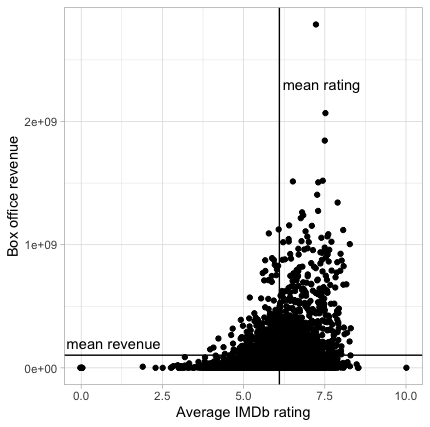
\includegraphics{movie dist.png}
    \caption{The distribution of movies by revenue and rating. The ``mean rating" and ``mean revenue" lines delineate movie categories.}
    \label{fig:my_label}
\end{figure}

\begin{table}[t]
\centering
\begin{tabular}{c|c}
  Algorithm   &  Mean Misclassification Error \\
  \hline \hline
    Decision Trees & 0.5447942 \\
    \hline
    Log Regression & 0.5338983 \\
    \hline
    Neural Network & 0.4794189 \\
    \hline
    Naive Bayes & 0.5690073 \\
    \hline
    kNN & 0.4939467 \\
    \hline
    SVM & 0.5484262 \\ 
    \hline
\end{tabular}
\caption{Mean misclassification errors for each prediction algorithm, using ``intuitive" movie categories as the target variable.}
\label{table 1}
\end{table}


\begin{table}[t]
\centering
\begin{tabular}{c|c}
  Algorithm   &  Mean Misclassification Error \\
  \hline \hline
    Decision Trees & 0.2442244 \\
    \hline
    Log Regression & 0.2376238  \\
    \hline
    Neural Network & 0.2359736  \\
    \hline
    Naive Bayes & 0.9191419 \\
    \hline
    kNN & 0.2475248 \\
    \hline
    SVM & 0.2293729   \\ 
    \hline
\end{tabular}
\caption{Mean misclassification errors for each prediction algorithm, using k-means clustering class as the target variable.}
\label{table 2}
\end{table}

\pagebreak
\appendix
\appendixpage
\section{Movie Metadata Variables}
\begin{singlespace}
\begin{itemize}
         \item whether the movie is "adult"
        \item which "collection" or series it belongs to, if any (e.g. Toy Story)
        \item its budget
        \item its genre(s)
        \item its language
        \item its original title
        \item production company
        \item production country
        \item release date
        \item revenue
        \item runtime
        \item which languages are spoken in the film
        \item status (e.g. released, in production)
        \item its tagline
        \item its title
        \item average IMDb rating
        \item how many ratings it has received on IMDb
        \item an overview (summary) of the movie
\end{itemize}
\end{singlespace}
\end{document}
